\documentclass{article}

\usepackage{graphicx}

\topmargin=-0.5cm
\leftmargin=-2cm
\rightmargin=0cm
\oddsidemargin=0cm
\evensidemargin=2cm
\textwidth=16.5cm
\textheight=20cm

\pagestyle{plain}

\begin{document}

\large

\vbox{}
\vspace{-2cm}
\begin{figure}[!ht]
%\hspace{-4mm}

\includegraphics[width=8cm]{img/logo.png}
\vspace{4mm}
\end{figure}
\noindent
\begin{center}
{\Huge Electrostatics Module}\\[2mm]
Based on Hermes2D ({\tt http://hpfem.org/hermes})\\[6mm]
\end{center}
\section{Module Description}

The electrostatics module calculates the distribution of the electric 
potential $\varphi$ induced by stationary electric charges. For charged 
objects one can specify either their voltage or the surface charge density.
Various objects and/or subdomains can have different values of the relative 
electric permittivity $\epsilon$.

The example below shows a 2D model of an oscilloscope that consists of
two electrodes (in the left part of the image) and a metallic screen (on the right). 
The voltage on the upper and lower electrode is 2000 V and 0 V, respectively,
The screen has zero surface charge density $\sigma$ and electric permittivity 
$\epsilon = 2$. Electric permittivity of the surrounding air is $\epsilon = 1$.\\
 

\begin{figure}[!ht]
\begin{center}
%\hspace{-4mm}
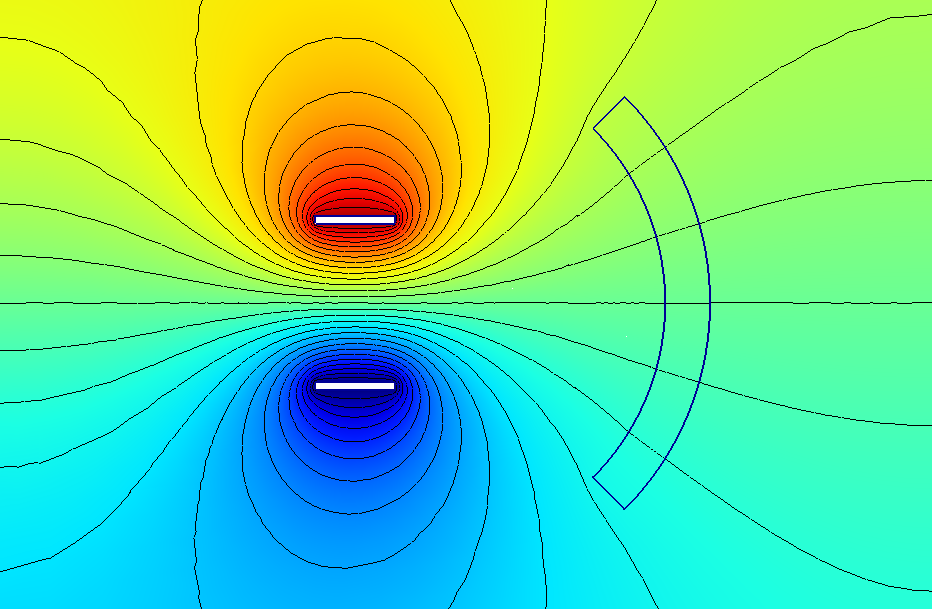
\includegraphics[width=10cm]{img/oscillo.png}
\caption{Electric field of an oscilloscope.}
\vspace{4mm}
\end{center}
\end{figure}
\noindent


\section{Underlying Equations}

The equation for the electric potential $\varphi$ is 

$$
-\mbox{div}(\epsilon \nabla \varphi) = \varrho
$$
where $\varrho$ is electric charge density. Once the electric potential 
$\varphi$ is calculated, the electric field vector $E$ can be obtained
as its negative gradient,

$$
E = -\nabla \varphi.
$$

\section{Boundary Conditions}

The following two types of boundary conditions are typical for electrostatics calculations:
\begin{itemize}
\item {\em Fixed voltage}: $\varphi = \varphi^*$ where $\varphi^*$ is a constant.
      Various objects in the arrangement can have different voltages. Grounded objects 
      usually have $\varphi = 0$ V (such as the lower electrode in the above example).
\item {\em Surface charge density}: $\sigma = \sigma^*$ where $\sigma^*$ is a constant.
      Various objects in the arrangement can have different values of $\sigma$. Objects 
      that do not carry any surface charges have $\sigma = 0$ C/m$^2$ (such as the screen 
      in the above example). 
\end{itemize}


\end{document}

